\documentclass[12pt, letterpaper]{article}
\usepackage[margin=.5in]{geometry}
\usepackage{graphicx}
\usepackage{tikz}

\title{
	GV101 Intro to PolSci\\
	\large{Professor Simon Hix}\\
	\large{Short Answer Questions Revision Document}
}
\author{Cedric Tan}
\date{April 2019}


\begin{document}
\maketitle
\abstract{This document covers the 8 topics that could be asked in the short answer section of the GV101 paper. There is a section dedicated to each topic and each section will begin with the definitions related to the subject then go into moderate depth on the relevant material before concluding with a half page summary on the topic. 

Note that this is a collation of readings, lecture notes and further supplementary material that can be found online. All work is not necessarily authentic and has been modified by me to fit my needs for this course}

\newpage
\tableofcontents
\newpage


\section{The Modernisation Theory of Democratisation}

\textbf{Definition:} Classic modernisation theory argues that countries are more likely to become democratic and stay democratic as they develop economically $\rightarrow$ this theory is more prevalent in high-income countries. (Clark, Golder and Golder 2017)

\subsection{Key Ideas}
Modernisation theory argues that all societies pass through the same historical stages of economic development. Those who are not democratic are simply \textbf{labelled as underdeveloped.} Rostow (1960) and Gerschenkron (1962) believed that African, Asian and Latin American countries were simply underdeveloped versions of countries in Europe.

These 'primitive' countries were characterised by large agricultural sectors and small industrial and service sectors. Eventually these countries are supposed to modernise by expanding their industrial and service sectors while reducing their emphasis on the level of agriculture.

\subsection{The Political Science Approach}
Helmed by Lipset (1959, 1960), modern societies, he says, need an appropriate type of government. Przeworski (1998, 2000) states that dictatorships and other types of government are replaced by democracies because:
\begin{itemize}
	\item Social structure becomes more complex
	\item New groups emerge and organise along various lines
	\item Labour requires active cooperation by employees hence the system can no longer be \textbf{command driven.}
	\item Dictatorships lose control and effectiveness as:
		\begin{itemize}
			\item Technological change endows private information and autonomy
			\item Civil democratic society tends to emerge as a result
		\end{itemize}
\end{itemize}
Hence for Przeworski, modernisation theory highlights the idea that as a country develops economically, they will also democratise due to the plurality of opinions that are formed along with the independence individuals develop with their new information.

Lipset also argues that higher income countries will also tend to maintain their democratic status as:
\begin{itemize}
	\item Sustaining the democracy is done through the people and their interests
	\item Interest in democracy is a main concern for these people and it persists as long as Przeworksi's reasons of diverse social structure remain
\end{itemize}

\subsection{Summary of Modernisation Theory}
Summary to be independently written for extended revision.

\newpage
\section{The Selectorate Theory for Non-Democratic Regimes}

\textbf{Definition:} Selectorate theory helps to explain why we observe tremendous variation in the economic performance of dictatorships. Rather than categorise governments as either democratic or dictatorial, selectorate theory characterises all governments by their location in a two-dimensional institutional space:
\begin{itemize}
	\item One dimension is the size of the selectorate: those with a say in selecting the leader
	\item The second is the size of the winning coalition: those in the selectorate whose support is essential for the leader to stay in office
\end{itemize}

\begin{center}
	$W = Winning\;Coalition$ and $S = Selectorate$
\end{center}

\subsection{Types of Selectorate and Winning Coalition}
Here are various forms of the relationship between Selectorate and Winning Coalition:
\begin{itemize}
	\item Large W and Large S
		\begin{itemize}
			\item Democracies usually
			\item Incentive to produce public goods
			\item Good government performance
			\item High levels of wealth, efficient governane and low rates of corruption and kleptocracy
		\end{itemize}
	\item Small W and Large S
		\begin{itemize}
			\item Personalist dictatorships and dominant party democracies
			\item Incentives to provide rewards to their relatively small winning coalition to stay in power
			\item Rigged voting hence the large selectorate but small winning coalition
			\item Poor government performance
			\item Low levels of wealth, inefficient governance with high levels of corruption and kleptocracy
		\end{itemize}
	\item Small W and Small S
		\begin{itemize}
			\item Monarchic and military dictatorships
			\item Produces middling government performance
			\item Moderate levels of corruption and kleptocracy
		\end{itemize}
\end{itemize}

The basic assumption of selectorate theory is that all political leaders are motivated by the desire to gain office. The competitive nature of politics forces all leaders to behave in this way. With that in mind, government performance is derivative of the ruling power making their selectorate happy. As shown above, personalistic or dominant party regimes will have lacking performance due to a small W that needs to be appeased. Dictatorships tend to focus on private goods to be given to their W as a result of this. For democracys, who have large Ws, public goods are the focus.

\subsection{Loyalty Norm}
The \textbf{Loyalty Norm} extends the idea of keeping the respective Ws happy. The Loyalty Norm is determined by $W/S$ which is effectively the probability that someone in the selectorate is in the winning coalition. \\

\textbf{Low Probability:}

There is less chance of a member of W defecting as the odds that they could form a new winning coalition is low, hence the loyalty here is high. Strong loyalty norm regimes tend to have a \textbf{greater chance in engaging in corruption and kleptocracy.} The amount to pay W is lower to keep their loyalty. \\

\textbf{High Probability:}

These is a higher chance of a member of W defecting as the odds that they could form a new winning coalition is high, hence the loyalty here is low. Low loyalty norm regimes tend to have a \textbf{lower chance in engaging in corruption and kleptocracy.} The amount required to pay W is higher to keep their loyalty. 

\begin{center}

We can recognise the probabilities by constructing a simple equation:

% insert equation and example from Clark, Golder and Golder
$R_L = Reward\;for\;Loyalty$ ;
$R_D = Reward\;for\;Defecting$ \\
$P_L = Probablity\;of\;Staying$ ;
$P_D = Probability\;of\;Defecting$ \\

\end{center}

\subsection{Size of the Winning Coalition}
The size of W can affect the eocnomic performance heavily through either investment into public or private goods. Leaders \textbf{always prefer to use private goods to satisfy the winning coalition rather than public goods} as it is easier and more effective. However, \textbf{increasing W should lead to more public good production.} This is simply because there is more people to please and public goods, since they are \textbf{non-rivalrous} \textit{(one person's consumption does not hinder another's ability to consume)} and \textbf{non-excludable} \textit{(one cannot prevent another from accessing this good entirely)}, appease everyone. Private goods, on the other hand, can only entertain a few people and so would not be able to maintain W.

\subsection{Summary of Selectorate Theory}
Summary to be independently written for extended revision.


\newpage
\section{Differences between Strategic and Expressive Voting}
\textbf{Definitions:}
\begin{itemize}
	\item \textbf{Strategic:} voting to produce an election outcome which is as close as possible to one's policy preferences (which may or may not mean voting for one's preferred party).
	\item \textbf{Expressive or Sincere:} voting on the basis of party attachment, political ideology or social group membership.
\end{itemize}

The two are often the same i.e. expressively voting is usually strategic voting as well. However, the interesting scenario is when one is \textbf{cross-pressured:} where voting one way means not voting the other way, \textbf{when the two styles of voting are mutually exclusive.}

Voters are assumed to be in a spatial model of politics where each voter has preferences about a range of policies. These preferences are \textbf{single peaked} which means that each voter has an \textbf{ideal point} in a single or multi-dimensional policy space.

\subsection{Expressive}
So as we noted before, expressive means:
\begin{itemize}
	\item Identification with a particular social cleavage, group or ideology
	\item People voting in line with this identity whether it be socio-economic class, ethnic or cultural associations
	\item Religion (Tilley 2015) may also have an effect on how one would vote
	\item Voting for whatever party feels \textbf{closest to me.}
\end{itemize}

Hence, voting expressively is pretty self-explanatory. It is because it is closest to your personal preference that you would vote in that way. If you vote purely in terms of expression, strategic voting does not matter whatsoever. When you are cross-pressured, you will choose the party closest to you.

\subsection{Strategic}
And for strategic we see that:
\begin{itemize}
	\item Citizens vote to try to influence the outcome of an election
	\item Overall policy outcomes that they attempt to influence would be closest to their ideal policy of all the likely outcomes
	\item Citizens attempt to influence outcomes whilst maintaining policy preferences close to their true preferences
\end{itemize}

\subsection{Why vote strategically?}
As opposed to expressive voting, the reasons for voting strategically can differ. Not that when we talked about cross-pressure, the expressive voter did not mind. However, for strategic voters, especially for those who support smaller parties, it is a serious problem as smaller party representatives are unlikely to be elected into office so strategic voters need to reconfigure their vote to influence a policy outcome.

There are two main reasons:
\begin{enumerate}
	\item \textbf{Local:} to influence the election outcome in a constituency. If the candidate a person most preferences has no chance of being elected, then vote for the closest candidate in preference from amongst the candidates who have a reasonable chance of winning. Example:
		\begin{itemize}
			\item British Elections
			\item First preference: Liberal Democrat
			\item \% Voting for Lib Dem as first preference: 56\%
			\item Likelihood is that the others split between Labour and Conservative
		\end{itemize}
	\item \textbf{National:} to influence the government formation and policy outcomes. If the party a person most prefers has no choice of influencing government formation or might form a coalition with a party which is further away from a person's preference, then vote for a party which is 'further away' but which will lead to a policy outcome closer to a person's ideal policy. Example:\\
	\begin{center}
		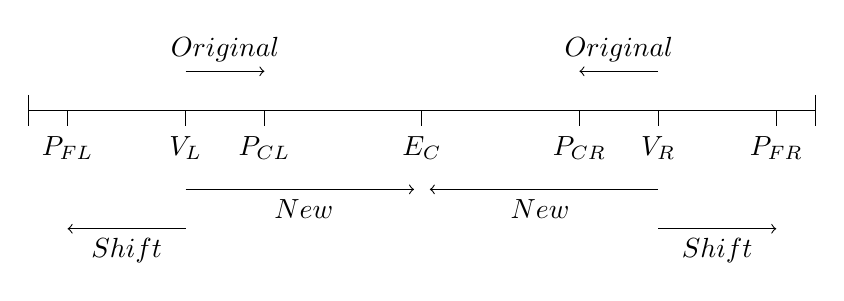
\begin{tikzpicture}
			\draw (-5,0) -- (5,0);
			\draw (-5, .2) -- (-5, -.2);
			\draw (5, .2) -- (5, -.2);
			\coordinate [label=below:$V_L$] (A) at (-3,-.2);
				\draw (-3, 0) -- (-3, -.2);
			\coordinate [label=below:$V_R$] (B) at (3,-.2);
				\draw (3, 0) -- (3, -.2);
			\coordinate [label=below:$E_C$] (C) at (0,-.2);
				\draw (0, 0) -- (0, -.2);
			\coordinate [label=below:$P_{CL}$] (D) at (-2,-.2);
				\draw (-2, 0) -- (-2, -.2);
			\coordinate [label=below:$P_{CR}$] (E) at (2,-.2);
				\draw (2, 0) -- (2, -.2);
			\coordinate [label=below:$P_{FL}$] (F) at (-4.5,-.2);
				\draw (-4.5, 0) -- (-4.5, -.2);
			\coordinate [label=below:$P_{FR}$] (G) at (4.5,-.2);
				\draw (4.5, 0) -- (4.5, -.2);
			\draw [->] (-3, .5) -- (-2, .5);
			\draw [->] (-3, -1) -- (-0.1, -1);
			\draw [->] (-3, -1.5) -- (-4.5, -1.5);
			\coordinate [label=above:${Original}$] (H) at (-2.5, .5);
			\coordinate [label=below:${New}$] (I) at (-1.5, -1);
			\coordinate [label=below:${Shift}$] (J) at (-3.75, -1.5);
			\draw [->] (3, .5) -- (2, .5);
			\draw [->] (3, -1) -- (0.1, -1);
			\draw [->] (3, -1.5) -- (4.5, -1.5);
			\coordinate [label=above:${Original}$] (K) at (2.5, .5);
			\coordinate [label=below:${New}$] (L) at (1.5, -1);
			\coordinate [label=below:${Shift}$] (M) at (3.75, -1.5);
		\end{tikzpicture}
	\end{center}
	
	Hence this result illustrates a shift in voting as a result of a delcared coalition that was further away from the voter's original preferences. Look at $V_L$ which is the left voter and $V_R$ which is the right voter, they would originally vote for the parties on the center-left and center-right respectively. However, after a coalition is announced between those two parties, the new distance from their true preferences is shifted all the way to the middle. They will subsequently shift their vote for the far left and far right parties, although further away, to see some compromise on policy preferences.
\end{enumerate}

\subsection{Summary of Expressive and Strategic Voting}


\newpage
\section{Down's Theory of Party Competition}
\textbf{Definition:} the simple Downsian model of two-party competition under plurality is generally characterised as predicting party convergence to the policy position espoused by the median voter.

\subsection{Assumption of the Downsian Model}
Below are a list of assumptions that Grofman (2004) thinks Downs has
\begin{enumerate}
	\item The system only has two political parties
	\item Single-round election for any office
	\item The election chooses a single candidate
	\item Elections take place within a single constituency
	\item The election is decided by a plurality vote
	\item Policies can be located a single left-right dimension
	\item Candidate policy positions are well defined
	\item Candidate policy positions are accurately estimated by each voter
	\item Voters look no further than the next decision
	\item Eligible voters go to the polls if the expected benefits of their vote's contribution to the election exceeds costs
	\item Voters care only about which candidate/party will enact policies closest to their preference location. If there are no policy differences, they are equally likely to support each and every candidate
	\item Parties/candidates care only about winning
	\item Parties/candidates look no further than the next election
	\item Candidates/parties accurately estimate the policy preferences of voters, or at minimum, they can identify the location of the median voter overall or in each party
	\item Candidates are part of a unified party team
\end{enumerate}

\subsection{The Downsian Model}
Assuming that there is a normal distribution of voters, we can model the vote distribution and subsequent convergence as shown below:
\begin{center}
	\begin{tikzpicture}
		\coordinate [label=left:$L$] (A) at (-5, 0);
		\coordinate (B) at (0, 6);
		\coordinate [label=below:$P_A$] (P_A) at (-3, 0);
		\coordinate [label=below:$P_B$] (P_B) at (0, 0);
		\coordinate [label=below:$Split$] (M_P) at (-1.5, 0);
		\coordinate (C) at (0, 0);
		\coordinate [label=right:$R$](D) at (5, 0);
		\draw [thick, dashed] (C) -- (B);
		\draw [thick](A) -- (D);
		\draw (M_P) -- (-1.5 , 5);
		\draw (A) .. controls (0, 7) .. (D);
		\coordinate [label=left:$Vote\;Share$] (Top) at (-5, 6);
		\draw [thick, ->](A) -- (Top);
	\end{tikzpicture}
\end{center}

From the picture above, we can see that the split vote share is given mostly to B as party B is on the median voter line. Hence, the voter base is split at the middle point between $P_A$ and $P_B$. For A to gain more voters, it needs to shift its policy position closer to B so that the split becomes more even. The Downsian model then predict that A will keep shifting until the party reaches the median voter like B. \textbf{It would be the same case if B started at a further right position and they both converged to the median voter. \textit{In game theory this would be called a Nash Equilibrium.}} This would end up looking as you would expect:
\begin{center}
	\begin{tikzpicture}
		\coordinate [label=left:$L$] (A) at (-5, 0);
		\coordinate (B) at (0, 6);
		\coordinate [label=below:$P_A$] (P_A) at (-3, 0);
		\draw [->] (-2.5, -.3) -- (-.9, -.3);
		\coordinate [label=below:$P_{AN}$] (P_AN) at (-0.3, 0);
		\coordinate [label=below:$P_B$] (P_B) at (0.3, 0);
		\coordinate (C) at (0, 0);
		\coordinate [label=right:$R$](D) at (5, 0);
		\draw [thick, dashed] (C) -- (B);
		\draw [thick](A) -- (D);
		\draw (A) .. controls (0, 7) .. (D);
		\coordinate [label=left:$Vote\;Share$] (Top) at (-5, 6);
		\draw [thick, ->] (A) -- (Top);
	\end{tikzpicture}
\end{center}

Thus, both parties have an equal share of the votes as shown by the diagram as $P_A$ shifts to $P_{AN}$.

\subsection{Reasons Why Parties Might Not Converge}
Below are some reasons that parties might not converge which you can be wary of:
\begin{itemize}
	\item Party positions are sticky due to the costs associated with moving
	\item There is threat of competition by flanks. Far right and Far left parties might arise as a result of Downsian convergence
	\item The reality of a multidimensional space, rather than the assumed single one, makes it more difficult to know where to move; it isn't always the median voter!
	\item Low turnout could happen since the fringes are not accounted for. It might be easier to mobilise your base than to capture new voters and persuade them to switch
	\item It is also dependent on how party leaders are chosen, whether it be the average voter, party officials or members which get to choose. This affects whether they are more extreme or moderate
 
\end{itemize}

\subsection{Summary of Downs Party Theory}

\newpage
\section{Olson's Theory of Collective Action}
\textbf{Definitions:} 
\begin{itemize}	
	\item \textbf{Collective Action:} refers to the pursuit of some objective by a group of individuals. Typically the objective is some form of public or private good.
	\item \textbf{Public Good:} a good which is non-excludable, whereby one cannot prevent other people from consuming the good once it is produced, and non-rivalrous, where one's consumption of the good does not affect another's ability to consume the same good.
	\item \textbf{Interest Group:} Any group which seeks to promote a particular policy or set of policies, and to organise to influence politics and policy-makers to achieve this policy.
	\item \textbf{Social Movement:} A large informal group of individuals and/or organisations which aim to promote a particular political or social issue, or promote/resist social change.

\end{itemize}

\subsection{The Logic of Collective Action}
Olson attempts to explain why some groups are more able to mobilise than others and, as a result, why public goods are likely to be undersupplied and private goods oversupplied. He presents us with a \textbf{collective action function} shown below:

\begin{center}
Each individual has a collective action function: \\
$R=(B \times P) - C$ \\
$R$ is the reward for participating in collective action \\
$B$ is the benefit of the good provided by a group \\
$P$ is the probability that the action of the individual makes a difference \\
$C$ is the cost of participation
\end{center}

\begin{center}
\textbf{Example 1: Student Demonstrations} \\
This example is to show the free rider problem we can face in collective action. \\
Taking $R=(B \times P) - C$ \\
$B$ would be cutting tuition fees \\
$P$ would be low as government probably won't change their stance \\
$C$ would be high as you're marching the whole day in the cold! \\
Hence we would have \\
$R=(B \times P) - C$ where $R<0$
\end{center}

Thus there's the free rider problem as individuals have little incentive to join a group which seeks a public good, as they all benefit if the protests are successful $\rightarrow$ there will be students protesting anyway. However, the costs for the individuals exceed the probable benefits.

\begin{center}
\textbf{Example 2: Farm Subsidies} \\
This example shows the power of organised interests \\
For this example, take 20 citizens in society with 4 out of the 20 being farmers. Each citizen \textbf{pays £1 in tax} and each farmer \textbf{receives a £5 subsidy.}

\begin{center}
\begin{tabular}{|c|c|c|c|}

	\hline
	& Tax & Subsidy & Outcome \\
	\hline
	\hline
	Farmers & £1 & £5 & +£4 \\
	\hline
	Individuals & £1 & £0 & -£1 \\
	\hline

\end{tabular}
\end{center}

Taking $R=(B \times P) - C$ \\
$B$ would be cutting tuition fees \\
$P$ would be low as government probably won't change their stance \\
$C$ would be high as you're marching the whole day in the cold! \\
Hence we would have \\
$R=(B \times P) - C$ where $R<0$
\end{center}

Each farmer has an incentive to organise to maintain subsidies while each taxpayer and consumer has no incentive to stop them. This is because farmers represent a concentrated interest seeking a \textbf{private good} while taxpayers represent a diffuse interest, \textbf{they are not aligned unless the tax is insanely high!} Hence farmers mobilise and more likely to get what they want.

\subsection{Summary of Olson's Theory of Collective Action}


\newpage
\section{Tsbelis' theory of veto-players and agenda setters}


\newpage
\section{Office vs Policy Seeking Theories of Coalitions}


\newpage
\section{Principal-Agent theory of Independent Institutions}


\end{document}